\documentclass[a4paper,12pt]{article}
%\usepackage{ctex}
\usepackage{graphicx}
\usepackage{hyperref}
\usepackage{geometry}
\usepackage{xcolor}
\usepackage{listings}
\usepackage{booktabs}
\usepackage{enumitem}
\usepackage{fancyhdr}
\usepackage{longtable}
\usepackage{float}
\usepackage{tikz}
\usetikzlibrary{arrows,shapes,positioning,calc}

\geometry{a4paper,left=2.5cm,right=2.5cm,top=2.5cm,bottom=2.5cm}

\hypersetup{
    colorlinks=true,
    linkcolor=blue,
    filecolor=magenta,      
    urlcolor=cyan,
    pdftitle={Requirement Analysis Specification Document},
    pdfpagemode=FullScreen,
}

\lstset{
    basicstyle=\ttfamily\small,
    breaklines=true,
    frame=single,
    xleftmargin=15pt,
    xrightmargin=15pt,
    backgroundcolor=\color{gray!10}
}

\title{Requirement Analysis Specification Document}
\author{Project Team}
\date{\today}

\pagestyle{fancy}
\fancyhf{}
\fancyhead[L]{Requirement Analysis Specification Document}
\fancyhead[R]{\thepage}
\fancyfoot[C]{Project Documentation}

\begin{document}

\maketitle
\tableofcontents
\newpage

\section{Document Overview}

\subsection{Document Purpose}

This document is the requirement analysis specification document for the project, aiming to provide a detailed description of the system's functional requirements, non-functional requirements, use case analysis, and module interaction relationships, serving as the foundation for subsequent design and development work. It clearly defines user requirements and transforms these requirements into implementable technical specifications. Additionally, through use case diagrams, it describes the responsibilities of the System group in the project and its interaction relationships with other groups (UI group, Data group, and Analysis group), providing clear role definitions and collaboration guidelines for all project stakeholders.

\subsection{Project Background}

This project aims to develop a comprehensive system with four main components working together: the System group, User Interface group (UI), Data group, and Analysis group. These four groups each have their specific responsibilities, working together to build a complete solution to meet user needs and business objectives. The System group, as the technical infrastructure provider of the project, is the designer and implementer of the project's technical architecture, responsible for the development of core system functionalities.

\subsection{Target Audience}

This document is intended for the following readers:
\begin{itemize}
  \item Project managers: To understand the overall project requirements and scope
  \item Development team members: To understand specific technical requirements and implementation details
  \item Testers: To develop test plans and test cases
  \item User representatives: To confirm whether the system meets business requirements
\end{itemize}

\subsection{References}

\begin{enumerate}
  \item Claude 3.7
  \item QwQ
\end{enumerate}

\section{System Overview}

\subsection{System Objectives}

This system aims to [describe the main objectives and problems to be solved here].
By integrating user interface, system architecture, data processing, and analysis functions, it provides users with a comprehensive solution to improve work efficiency and decision-making quality.

\subsection{System Scope}

This system includes but is not limited to the following functional areas:
\begin{itemize}
  \item User interface display and interaction
  \item System core architecture and services
  \item Data collection, storage, and management
  \item Data analysis and visualization
\end{itemize}

\subsection{System Architecture Overview}

The system consists of four main components with the following responsibilities:

\begin{itemize}
  \item \textbf{System Group}: Responsible for core architecture design, API implementation, third-party service integration, system deployment, performance optimization, security assurance, and monitoring systems
  \item \textbf{User Interface Group (UI)}: Responsible for user interface design and implementation, user experience optimization, and front-end interaction with backend APIs
  \item \textbf{Data Group}: Responsible for data model design, database implementation, data processing workflows, and data quality assurance
  \item \textbf{Analysis Group}: Responsible for data analysis algorithms, report generation, data visualization, and decision support models
\end{itemize}

These components interact through well-defined interfaces, as shown in the following figure:

\begin{figure}[H]
    \centering
    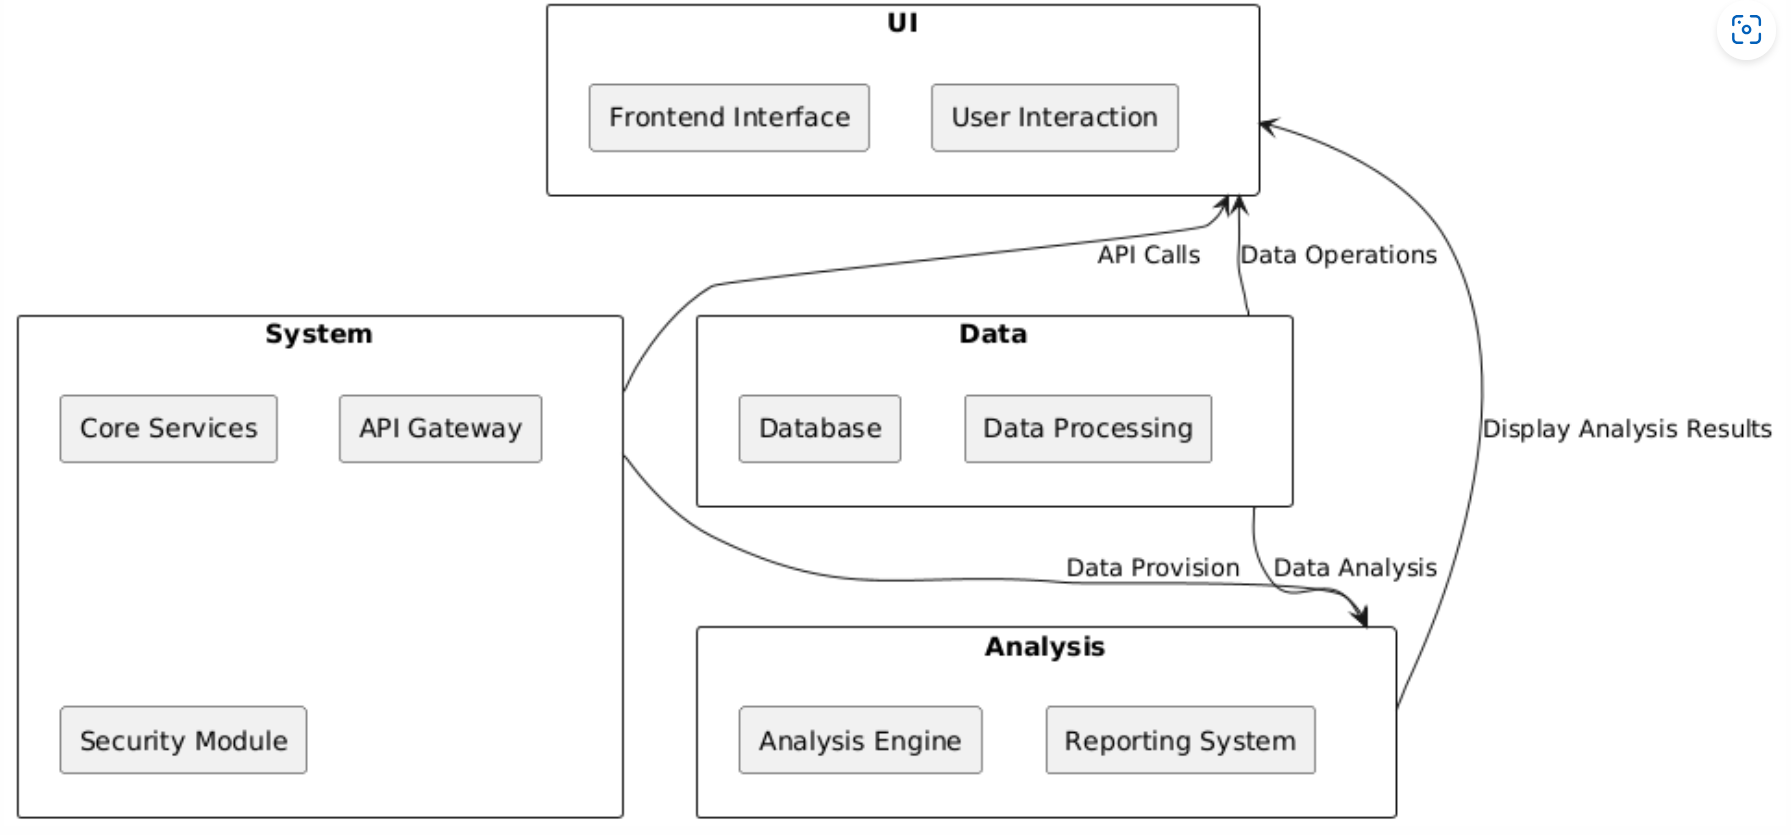
\includegraphics[width=0.75\linewidth]{assets/7_EG.png}
    \caption{System Architecture Overview}
    \label{fig:system-architecture}
\end{figure}

\section{User Requirements}

\subsection{User Role Definition}

The system identifies the following main user roles:

\begin{enumerate}
  \item \textbf{System Administrator}: Responsible for system management and maintenance
  \item \textbf{Doctor User}: Uses the main functions of the system
  \item \textbf{Patient User}: Uses some functions of the system
\end{enumerate}

\subsection{User Scenarios}

The following is an overview of the main user scenarios:

\begin{enumerate}
  \item User login and authentication
  \item Data entry and editing
  \item Data query and retrieval
  \item Data analysis and report generation
  \item System management and configuration
  \item Security auditing and monitoring
\end{enumerate}

\section{Functional Requirements}

\subsection{UI Group Functional Requirements}

\begin{enumerate}
  \item \textbf{User Interface Design}
  \begin{itemize}
    \item Design interface layouts that comply with user experience principles
    \item Implement responsive design to adapt to different devices
    \item Provide consistent visual style and component library
  \end{itemize}
  
  \item \textbf{User Interaction Implementation}
  \begin{itemize}
    \item Implement basic functions such as user login, registration, and password reset
    \item Provide personalization settings and theme customization
    \item Implement multi-language support
  \end{itemize}
  
  \item \textbf{Frontend Data Display}
  \begin{itemize}
    \item Implement data tables, charts, and other display components
    \item Provide data filtering, sorting, and pagination functions
    \item Support data export and printing
  \end{itemize}
\end{enumerate}

\subsection{System Group Functional Requirements}

The System group's main responsibility in the project is to serve as the technical infrastructure provider, responsible for the development of core system functionalities. The following are the specific functional requirements for the System group:

\begin{enumerate}
  \item \textbf{Build and Deployment Process}
  
  \begin{figure}[H]
    \centering
    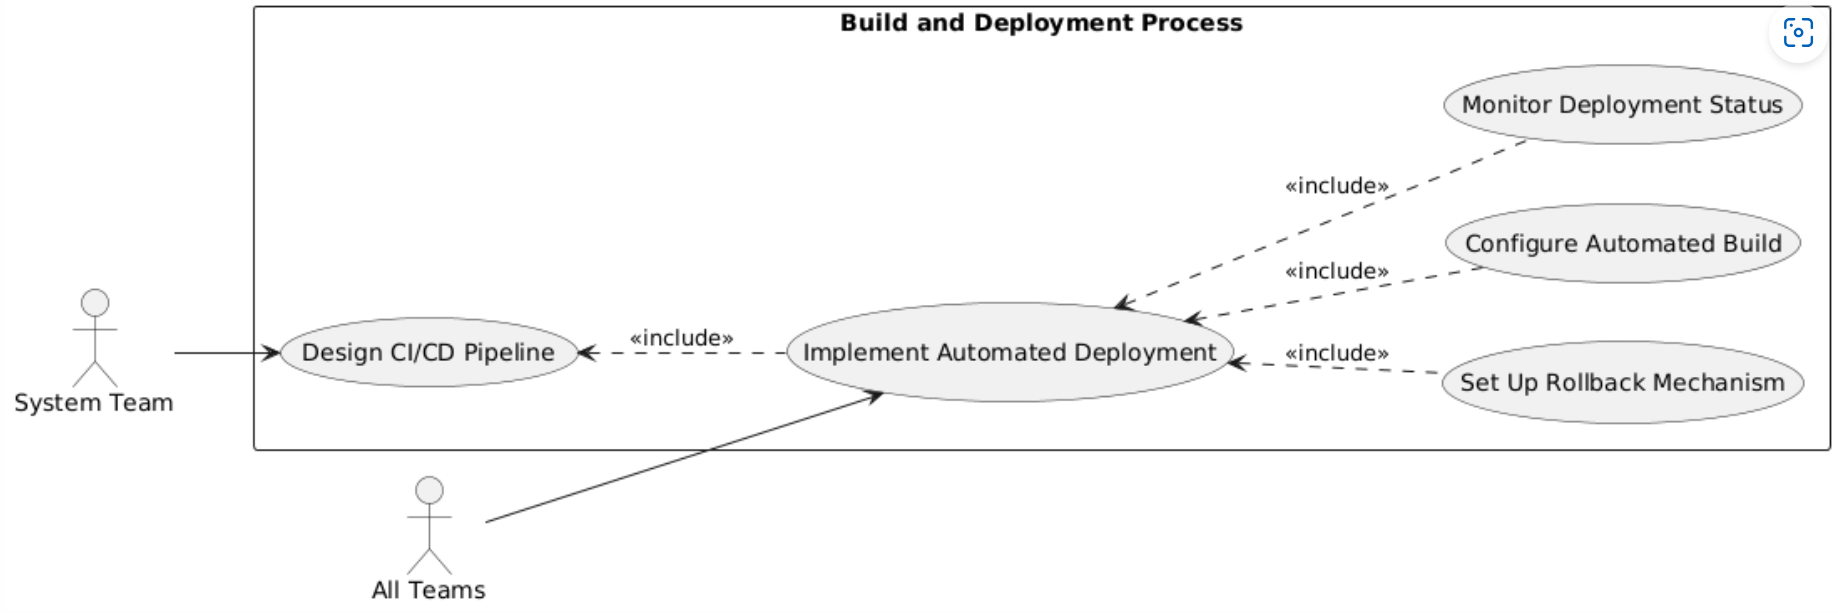
\includegraphics[width=0.9\linewidth]{assets/image1_EG.png}
    \caption{Build and Deployment Process Use Case Diagram}
    \label{fig:deployment-process}
  \end{figure}
  
  \begin{itemize}
    \item Design and implement complete CI/CD processes
    \item Configure automated build and test environments
    \item Provide deployment status monitoring
    \item Establish rollback mechanisms for deployment failures
  \end{itemize}
  
  \item \textbf{Integrate Third-party Services}
  
  \begin{figure}[H]
    \centering
    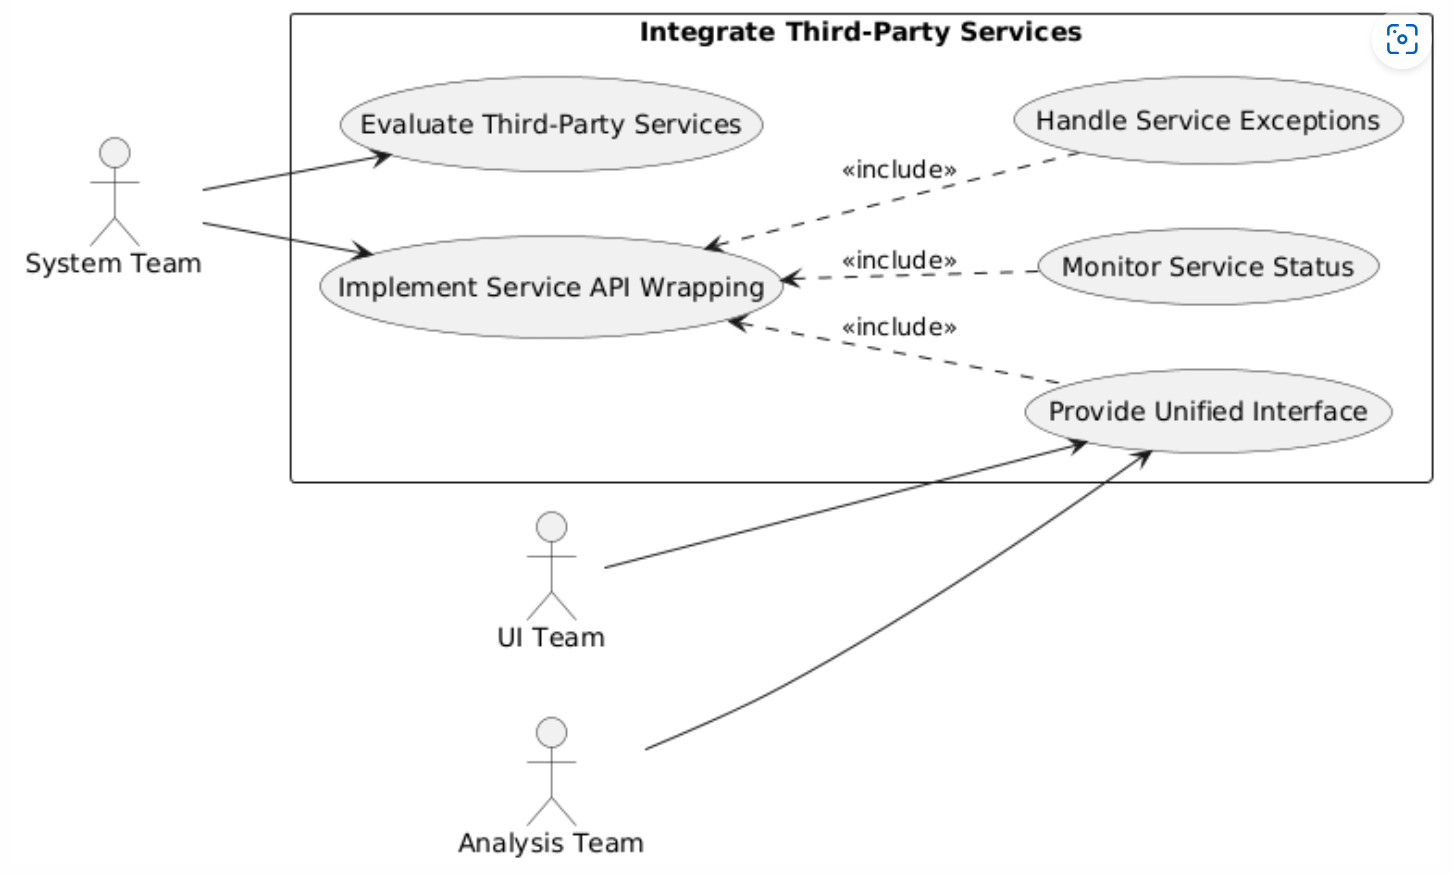
\includegraphics[width=0.75\linewidth]{assets/image11_EG.png}
    \caption{Third-party Service Integration Use Case Diagram}
    \label{fig:third-party-services}
  \end{figure}
  
  \begin{itemize}
    \item Evaluate and select third-party services suitable for project requirements
    \item Implement encapsulation of third-party APIs
    \item Provide unified interface specifications
    \item Handle third-party service exceptions
    \item Monitor third-party service availability and performance
  \end{itemize}
  
  \item \textbf{Collaborative Database Development}
  
  \begin{figure}[H]
    \centering
    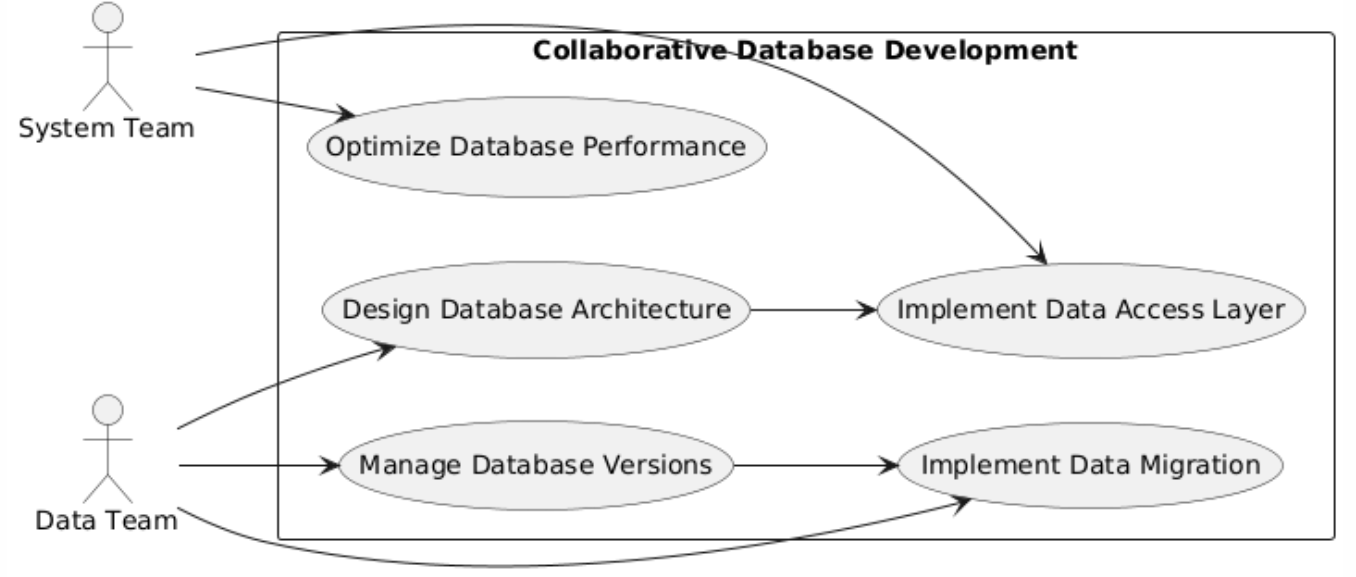
\includegraphics[width=0.75\linewidth]{assets/image8_EG.png}
    \caption{Collaborative Database Development Use Case Diagram}
    \label{fig:database-development}
  \end{figure}
  
  \begin{itemize}
    \item Collaborate with the Data group to implement data access layer
    \item Optimize database performance
    \item Implement data caching mechanisms
  \end{itemize}
  
  \item \textbf{API Design and Implementation}
  
  \begin{figure}[H]
    \centering
    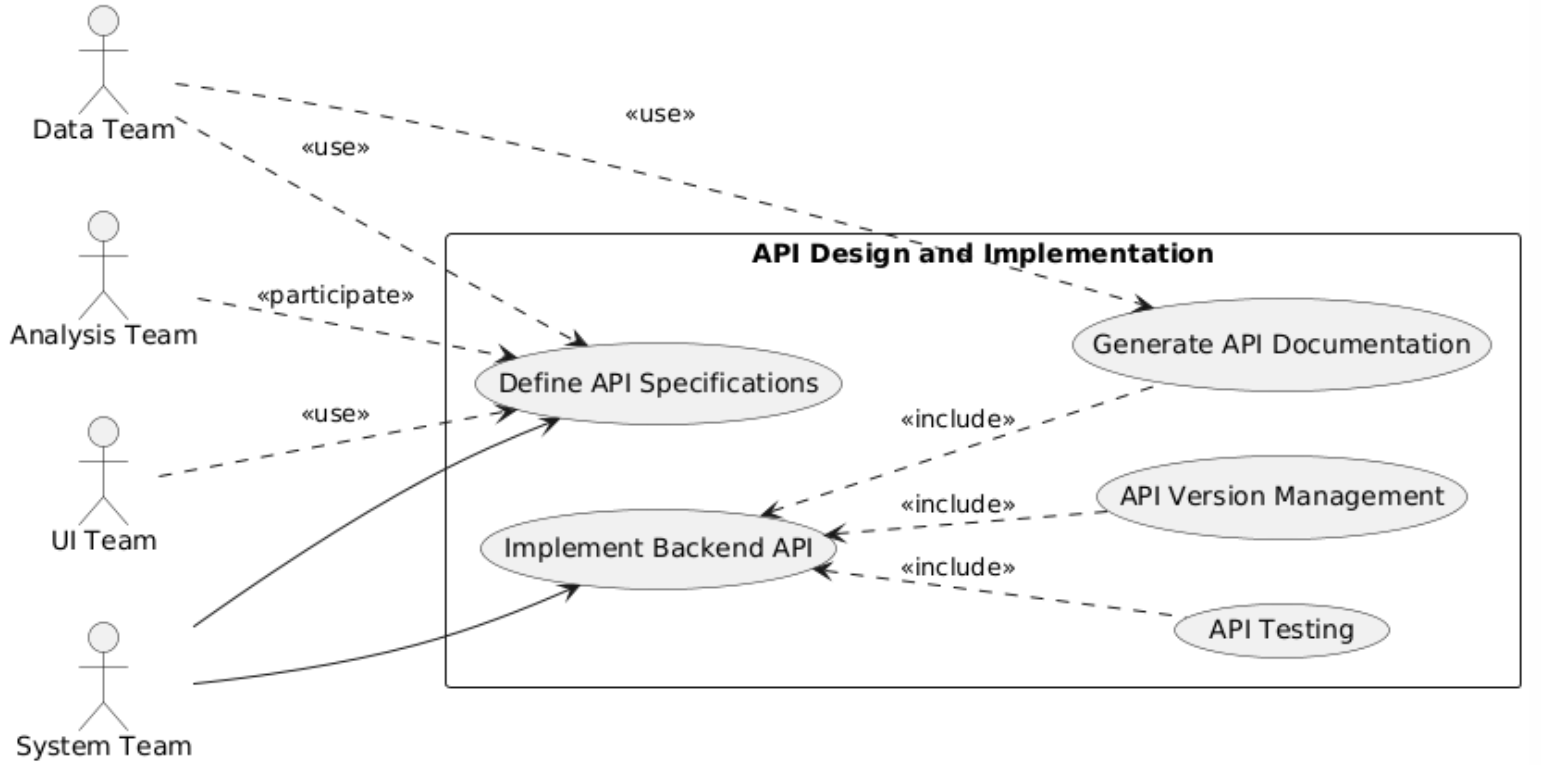
\includegraphics[width=0.75\linewidth]{assets/image4_EG.png}
    \caption{API Design and Implementation Use Case Diagram}
    \label{fig:api-design}
  \end{figure}
  
  \begin{itemize}
    \item Develop API design standards and specifications
    \item Implement all backend API functionalities
    \item Generate complete API documentation
    \item Conduct API unit testing and integration testing
    \item Manage API versions and compatibility
  \end{itemize}
  
  \item \textbf{Performance Optimization}
  
  \begin{figure}[H]
    \centering
    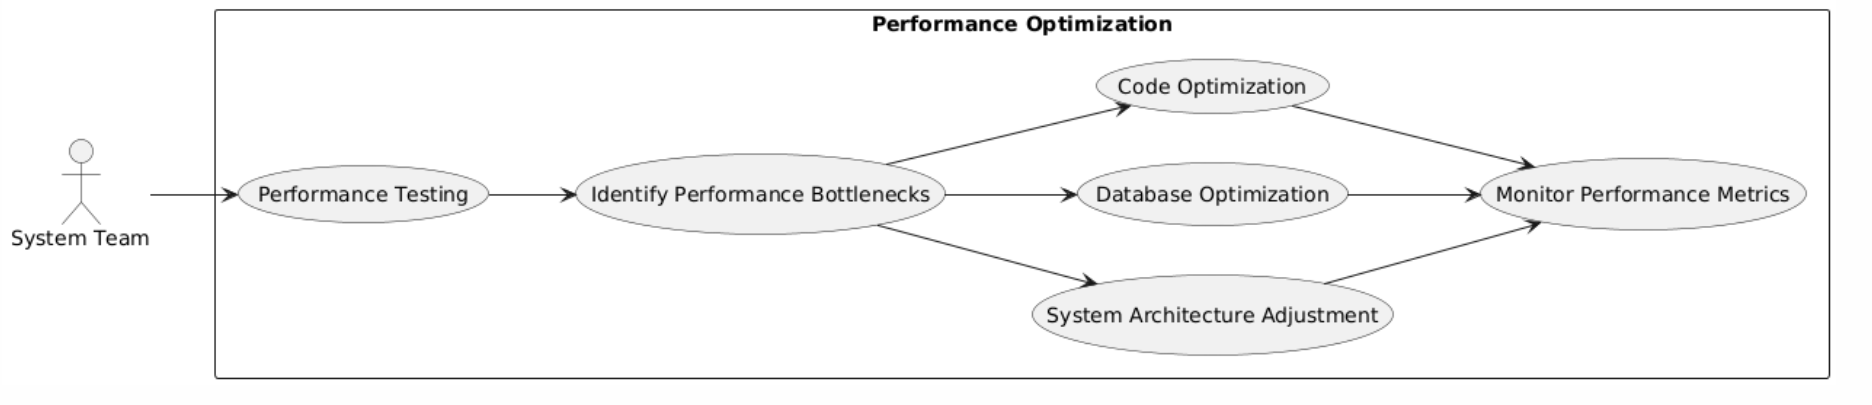
\includegraphics[width=0.75\linewidth]{assets/image5_EG.png}
    \caption{Performance Optimization Use Case Diagram}
    \label{fig:performance-optimization}
  \end{figure}
  
  \begin{itemize}
    \item Design and execute performance testing plans
    \item Analyze and identify system performance bottlenecks
    \item Optimize code execution efficiency
    \item Collaborate with the Data group on database performance optimization
    \item Adjust system architecture when necessary
    \item Continuously monitor system performance metrics
  \end{itemize}
  
  \item \textbf{Security Assurance}
  
  \begin{figure}[H]
    \centering
    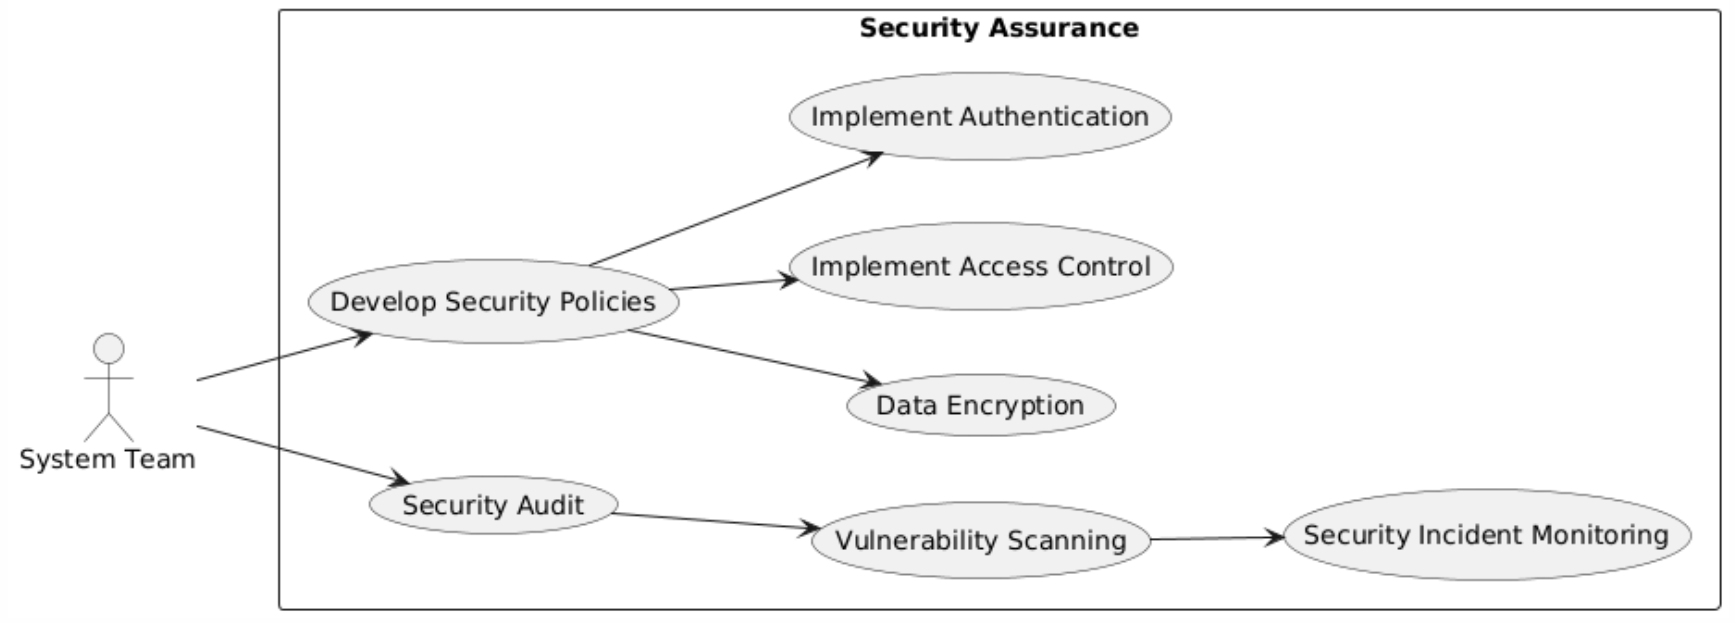
\includegraphics[width=0.75\linewidth]{assets/image6_EG.png}
    \caption{Security Assurance Use Case Diagram}
    \label{fig:security-protection}
  \end{figure}
  
  \begin{itemize}
    \item Develop system security policies and standards
    \item Implement identity authentication and authorization mechanisms
    \item Implement fine-grained permission control
    \item Encrypt sensitive data storage and transmission
    \item Prevent common security threats (SQL injection, XSS, etc.)
    \item Conduct regular security audits and vulnerability scanning
    \item Implement security event monitoring and response mechanisms
  \end{itemize}
  
  \item \textbf{Monitoring and Logging System}
  
  \begin{figure}[H]
    \centering
    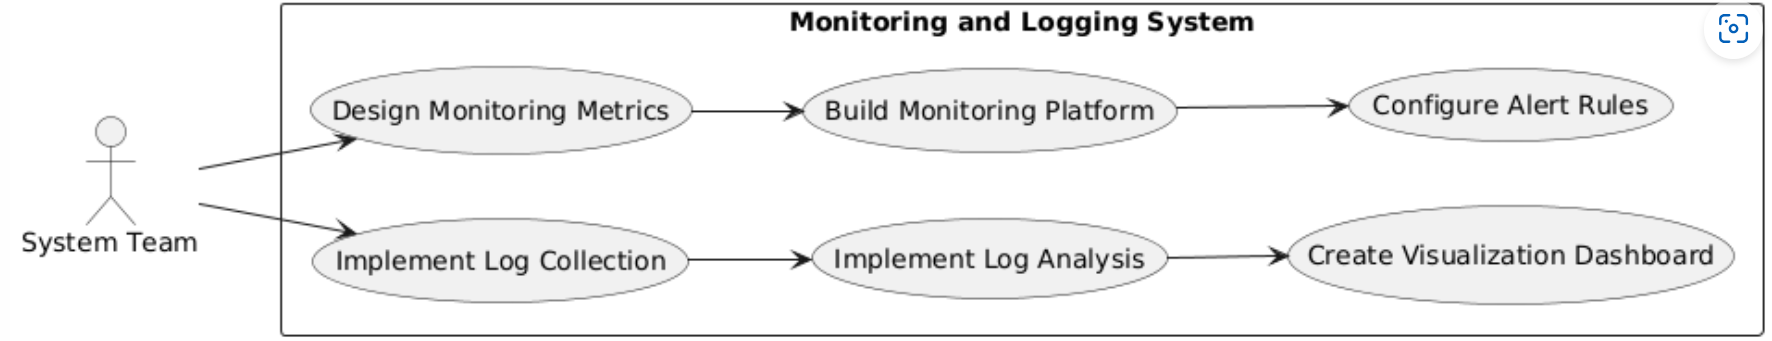
\includegraphics[width=0.75\linewidth]{assets/image7_EG.png}
    \caption{Monitoring and Logging System Use Case Diagram}
    \label{fig:monitoring-logging}
  \end{figure}
  
  \begin{itemize}
    \item Design system key monitoring metrics
    \item Implement comprehensive log collection mechanisms
    \item Build unified monitoring platform
    \item Configure reasonable alert rules
    \item Implement log aggregation and analysis functions
    \item Create intuitive visualization dashboards
  \end{itemize}
\end{enumerate}

\subsection{Data Group Functional Requirements}

\begin{enumerate}
  \item \textbf{Database Design}
  \begin{itemize}
    \item Design database models and table structures
    \item Define data constraints and relationships
    \item Implement data version control
  \end{itemize}
  
  \item \textbf{Data Processing Workflow}
  \begin{itemize}
    \item Implement data ETL (Extract, Transform, Load) processes
    \item Provide data batch import and export functions
    \item Implement data cleaning and validation mechanisms
  \end{itemize}
  
  \item \textbf{Data Quality Management}
  \begin{itemize}
    \item Implement data quality check rules
    \item Monitor data integrity and consistency
    \item Provide data repair tools
  \end{itemize}
\end{enumerate}

\subsection{Analysis Group Functional Requirements}

\begin{enumerate}
  \item \textbf{Data Analysis Algorithms}
  \begin{itemize}
    \item Implement statistical analysis functions
    \item Provide predictive analysis models
    \item Support custom analysis rules
  \end{itemize}
  
  \item \textbf{Report Generation}
  \begin{itemize}
    \item Design standard report templates
    \item Support custom reports
    \item Implement scheduled report generation and distribution
  \end{itemize}
  
  \item \textbf{Data Visualization}
  \begin{itemize}
    \item Provide various charts and visualization components
    \item Support interactive data exploration
    \item Implement data drilling and aggregation analysis
  \end{itemize}
\end{enumerate}

\section{Non-functional Requirements}

\subsection{Performance Requirements}

\begin{enumerate}
  \item \textbf{Response Time}
  \begin{itemize}
    \item Page loading time should not exceed 3 seconds
    \item API interface response time should not exceed 1 second
    \item Report generation time should not exceed 5 seconds
  \end{itemize}
  
  \item \textbf{Concurrent Processing}
  \begin{itemize}
    \item The system should support at least 100 concurrent users
    \item The database should handle 50 concurrent transactions simultaneously
  \end{itemize}
  
\end{enumerate}

\subsection{Reliability Requirements}

\begin{enumerate}
  
  \item \textbf{Data Backup and Recovery}
  \begin{itemize}
    \item Perform daily data backups
    \item Data recovery time should not exceed 4 hours
  \end{itemize}
  
  \item \textbf{Error Handling}
  \begin{itemize}
    \item The system should provide clear error messages
    \item Critical operations should provide rollback mechanisms
  \end{itemize}
\end{enumerate}

\subsection{Security Requirements}

\begin{enumerate}
  \item \textbf{Identity Authentication and Authorization}
  \begin{itemize}
    \item Implement multi-factor authentication
    \item Role-based access control
    \item Regular password update policies
  \end{itemize}
  
  \item \textbf{Data Security}
  \begin{itemize}
    \item Encrypt sensitive data storage
    \item Communication encryption (HTTPS)
  \end{itemize}
  
\end{enumerate}

\subsection{Maintainability Requirements}

\begin{enumerate}
  \item \textbf{Modular Design}
  \begin{itemize}
    \item The system should follow loose coupling and high cohesion design principles
    \item Support independent module updates and deployment
  \end{itemize}
  
  \item \textbf{Complete Documentation}
  \begin{itemize}
    \item Provide detailed system architecture documentation
    \item Write complete API documentation
    \item Maintain code comments and key algorithm descriptions
  \end{itemize}
  
  \item \textbf{Testability}
  \begin{itemize}
    \item Support automated unit testing and integration testing
    \item Provide testing environments and test data
  \end{itemize}
\end{enumerate}

\section{Use Case Analysis}

\subsection{System Group Use Case Overview}

The following use case diagram shows the System group's main responsibilities and interaction relationships with other groups:

\begin{figure}[H]
    \centering
    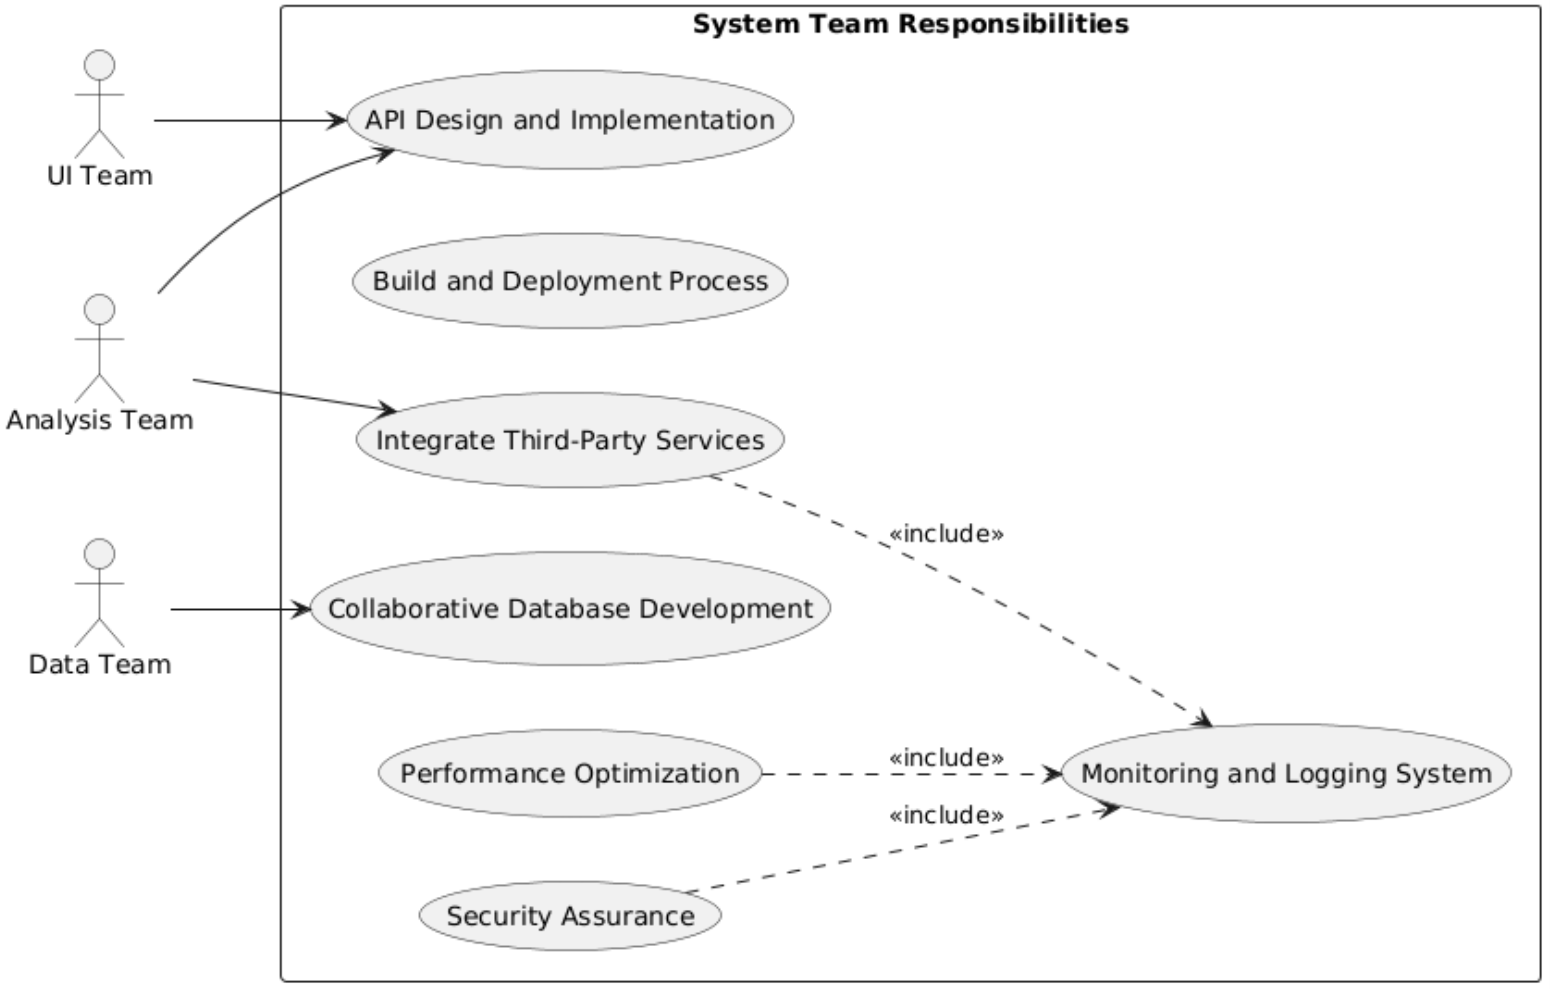
\includegraphics[width=0.75\linewidth]{assets/image2_EG.png}
    \caption{System Group Use Case Overview}
    \label{fig:system-overview}
\end{figure}

\subsection{System Group Use Case Analysis}

\subsubsection{Build and Deployment Process}

\textbf{Use Case Name}: Build and Deployment Process

\textbf{Actor}: System Group

\textbf{Preconditions}:
\begin{itemize}
  \item Project code repository has been established
  \item Deployment environment is ready
\end{itemize}

\textbf{Postconditions}:
\begin{itemize}
  \item Automated CI/CD process can run normally
  \item All groups can use the deployment process to deploy code
\end{itemize}

\textbf{Basic Flow}:
\begin{enumerate}
  \item System group designs CI/CD process
  \item Configure automated build environment
  \item Implement automated deployment mechanism
  \item Set up deployment monitoring and rollback mechanism
  \item All groups use the deployment process to deploy code
\end{enumerate}

\textbf{Alternative Flow}:
\begin{enumerate}
  \item When deployment fails, automatically trigger rollback mechanism
  \item When environment is unavailable, provide manual deployment options
\end{enumerate}

\textbf{Deliverables}:
\begin{itemize}
  \item CI/CD configuration files
  \item Deployment scripts
  \item Deployment documentation
\end{itemize}

\subsubsection{Integrate Third-party Services}

\textbf{Use Case Name}: Integrate Third-party Services

\textbf{Actor}: System Group

\textbf{Preconditions}:
\begin{itemize}
  \item Third-party services to be integrated have been identified
  \item Related API documentation and access permissions have been obtained
\end{itemize}

\textbf{Postconditions}:
\begin{itemize}
  \item Third-party services are successfully integrated into the system
  \item Provide unified interfaces for other groups to use
\end{itemize}

\textbf{Basic Flow}:
\begin{enumerate}
  \item Evaluate and select third-party services suitable for project requirements
  \item Implement encapsulation of third-party APIs
  \item Provide unified interface specifications
  \item Handle third-party service exceptions
  \item Monitor third-party service availability and performance
\end{enumerate}

\textbf{Alternative Flow}:
\begin{enumerate}
  \item When third-party services are unavailable, provide degradation strategies
  \item When interfaces change, provide compatibility handling
\end{enumerate}

\textbf{Deliverables}:
\begin{itemize}
  \item Third-party service integration documentation
  \item API encapsulation code
  \item Service configuration guide
\end{itemize}

\subsubsection{Collaborative Database Development}

\textbf{Use Case Name}: Collaborative Database Development

\textbf{Actor}: System Group and Data Group

\textbf{Preconditions}:
\begin{itemize}
  \item System requirements have been clarified
  \item Data requirements have been collected
\end{itemize}

\textbf{Postconditions}:
\begin{itemize}
  \item Database architecture design is completed
  \item Data version management mechanism is established
\end{itemize}

\textbf{Basic Flow}:
\begin{enumerate}
  \item Data group designs database architecture
  \item System group implements data access layer
  \item Data group manages database versions
  \item Data group implements data migration solutions
\end{enumerate}

\textbf{Alternative Flow}:
\begin{enumerate}
  \item When architecture design has issues, System group proposes modification suggestions
  \item When performance issues are serious, jointly redesign data models
\end{enumerate}

\textbf{Responsibility Division}:
\begin{itemize}
  \item System Group: Implement data access layer and database performance optimization
  \item Data Group: Responsible for database architecture design, version management, and data migration
\end{itemize}

\textbf{Deliverables}:
\begin{itemize}
  \item Database design documentation
  \item Database version control scripts
  \item Data access layer code
\end{itemize}

\subsubsection{API Design and Implementation}

\textbf{Use Case Name}: API Design and Implementation

\textbf{Actor}: System Group

\textbf{Preconditions}:
\begin{itemize}
  \item System functional requirements have been clarified
  \item Data models have been defined
\end{itemize}

\textbf{Postconditions}:
\begin{itemize}
  \item API interface design is completed and implemented
  \item API documentation is generated and published
  \item API testing is passed
\end{itemize}

\textbf{Basic Flow}:
\begin{enumerate}
  \item Develop API design standards and specifications
  \item Implement all backend API functionalities
  \item Generate complete API documentation
  \item Conduct API unit testing and integration testing
  \item Manage API versions and compatibility
\end{enumerate}

\textbf{Alternative Flow}:
\begin{enumerate}
  \item When requirements change, update API design and notify relevant parties
  \item When security vulnerabilities are discovered, promptly fix and update
\end{enumerate}

\textbf{Deliverables}:
\begin{itemize}
  \item API design documentation
  \item API implementation code
  \item API test cases
  \item Swagger/OpenAPI documentation
\end{itemize}

\subsubsection{Monitoring and Logging System}

\textbf{Use Case Name}: Monitoring and Logging System

\textbf{Actor}: System Group

\textbf{Preconditions}:
\begin{itemize}
  \item Basic system functions have been implemented
  \item Monitoring requirements and metrics have been determined
\end{itemize}

\textbf{Postconditions}:
\begin{itemize}
  \item Monitoring and logging system is established and running
  \item Exception alert mechanism is effective
\end{itemize}

\textbf{Basic Flow}:
\begin{enumerate}
  \item Design system key monitoring metrics
  \item Implement comprehensive log collection mechanisms
  \item Build unified monitoring platform
  \item Configure reasonable alert rules
  \item Implement log aggregation and analysis functions
  \item Create intuitive visualization dashboards
\end{enumerate}

\textbf{Alternative Flow}:
\begin{enumerate}
  \item When log volume is too large, implement log grading and sampling strategies
  \item When false alarms are too many, adjust alert thresholds and rules
\end{enumerate}

\textbf{Deliverables}:
\begin{itemize}
  \item Monitoring system configuration
  \item Log analysis platform
  \item Alert rule configuration
  \item Operation manual
\end{itemize}

\subsection{Other Key Use Cases}

This section supplements detailed descriptions of other key use cases as needed.

\section{Data Requirements}

\subsection{Data Entities}

The main data entities involved in the system include:

\begin{enumerate}
  \item \textbf{User}: Stores system user information
  \item \textbf{Role}: Defines user roles and permissions
  \item \textbf{Business Data}: [Supplement according to specific project]
  \item \textbf{Configuration Data}: System configuration and parameters
  \item \textbf{Log Data}: System operation and event logs
\end{enumerate}

\subsection{Data Dictionary}

The following is the field definition of the system's main data entities:

\begin{longtable}{|p{3cm}|p{3cm}|p{3cm}|p{6cm}|}
\hline
\textbf{Entity} & \textbf{Field} & \textbf{Type} & \textbf{Description} \\
\hline
\endhead
User & id & Integer & User unique identifier \\
\hline
 & username & String & Username \\
\hline
 & password & String & Encrypted password \\
\hline
 & email & String & User email \\
\hline
 & status & Enum & User status (Active/Disabled) \\
\hline
Role & id & Integer & Role unique identifier \\
\hline
 & name & String & Role name \\
\hline
 & permissions & String array & Permission list \\
\hline
\end{longtable}

\textbf{Note}: Supplement the complete data dictionary according to specific project requirements.

\subsection{Data Flow}

The main data flows of the system are as follows:

\begin{figure}[H]
    \centering
    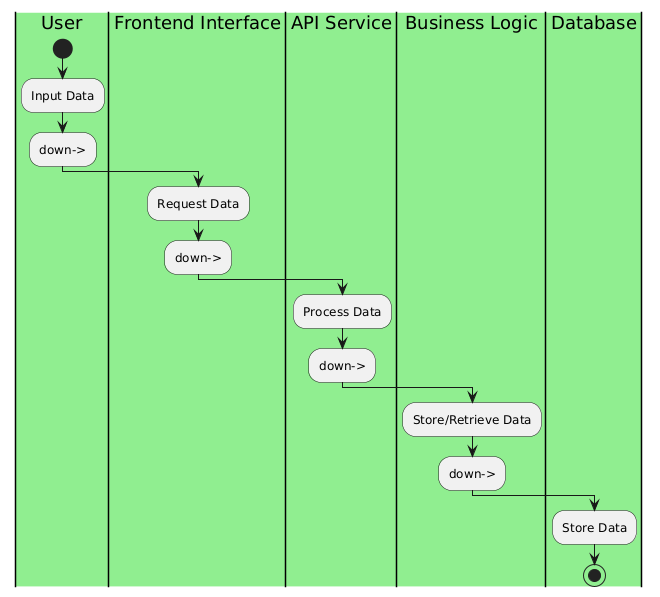
\includegraphics[width=0.75\linewidth]{assets/6_EG.png}
    \caption{Data Flow Diagram}
    \label{fig:data-flow}
\end{figure}

\section{Interface Requirements}

\subsection{System Group and Other Groups Interface Overview}

As the technical infrastructure provider of the project, the System group needs to establish clear interfaces with the UI group, Data group, and Analysis group to ensure smooth collaboration among all groups. The following diagram shows the main interface relationships between the System group and other groups:

\begin{figure}[H]
    \centering
    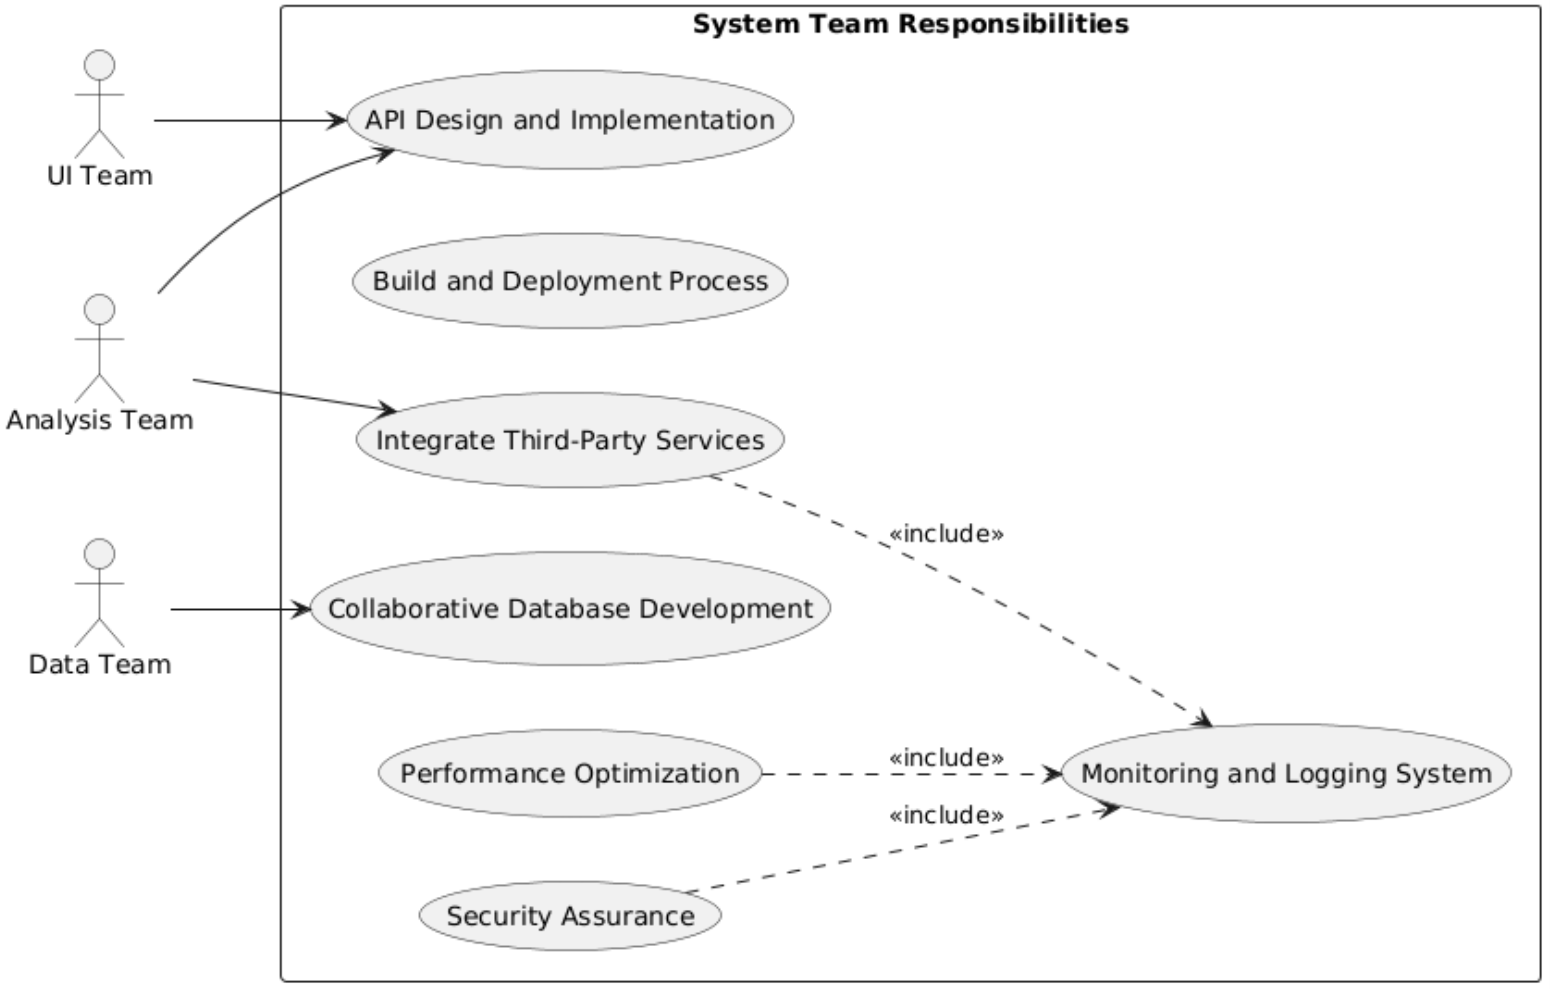
\includegraphics[width=0.8\linewidth]{assets/image2_EG.png}
    \caption{System Group and Other Groups Interface Relationship Diagram}
    \label{fig:interface-relations}
\end{figure}

\subsection{System Group and UI Group Interface}

The System group provides backend service support for the UI group, with interfaces mainly manifested at the API level.

\subsubsection{API Interface Specifications}

\begin{itemize}
  \item \textbf{Interface Style}: RESTful API
  \item \textbf{Data Format}: JSON
  \item \textbf{Authentication Method}: JWT (JSON Web Token)
  \item \textbf{Status Code Usage}: Follow HTTP standard status codes
  \item \textbf{Version Control}: Include version number in URL path, e.g., /api/v1/users
  \item \textbf{Error Handling}: Unified error response format
  \item \textbf{Pagination Mechanism}: Support limit/offset and cursor pagination
\end{itemize}

\subsubsection{Core API Interfaces}

\begin{longtable}{|p{3cm}|p{2.5cm}|p{2.5cm}|p{7cm}|}
\hline
\textbf{Interface Name} & \textbf{Request Method} & \textbf{Path} & \textbf{Description} \\
\hline
\endhead
User Authentication & POST & /api/v1/auth/login & UI group calls this interface for user login authentication \\
\hline
Get User Information & GET & /api/v1/users/profile & Get detailed information of the current logged-in user \\
\hline
Data Query & GET & /api/v1/data & Support various query parameters, return paginated data \\
\hline
Data Operations & POST/PUT/DELETE & /api/v1/data & Create, update, delete data \\
\hline
File Upload & POST & /api/v1/files & Support multi-file upload, return file URL \\
\hline
System Configuration & GET & /api/v1/config & Get system configuration parameters required by UI \\
\hline
\end{longtable}

\subsubsection{Frontend-Backend Interaction Process}

\begin{enumerate}
  \item \textbf{User Authentication Process}
  \begin{itemize}
    \item UI group collects user credentials (username/password)
    \item Call authentication API to obtain access token
    \item Subsequent requests carry token for identity verification
  \end{itemize}
  
  \item \textbf{Data Interaction Process}
  \begin{itemize}
    \item UI group constructs requests according to API specifications
    \item System group processes requests and returns appropriate responses
    \item UI group updates interface based on responses
  \end{itemize}
  
  \item \textbf{Error Handling Process}
  \begin{itemize}
    \item System group returns standard error codes and detailed error messages
    \item UI group displays appropriate error prompts based on error type
  \end{itemize}
\end{enumerate}

\subsection{System Group and Data Group Interface}

The System group and Data group closely collaborate in database development and data processing, with interface design considering data access efficiency and security.

\subsubsection{Database Access Interface}

\begin{itemize}
  \item \textbf{Data Access Pattern}: Repository pattern
  \item \textbf{ORM Framework}: Provide object-relational mapping capabilities
  \item \textbf{Transaction Support}: Support distributed transactions
  \item \textbf{Caching Mechanism}: Multi-level caching strategy
  \item \textbf{Connection Pool Management}: Optimize database connection resources
\end{itemize}

\subsubsection{Main Data Interaction Scenarios}

\begin{longtable}{|p{3cm}|p{4cm}|p{8cm}|}
\hline
\textbf{Interaction Scenario} & \textbf{Interface Method} & \textbf{Description} \\
\hline
\endhead
Data Query & findById(), findByCondition() & Support single record query and conditional query, Data group responsible for SQL optimization \\
\hline
Data Writing & save(), update(), delete() & Provide unified data writing interface, System group handles concurrency control \\
\hline
Batch Operations & batchInsert(), batchUpdate() & High-performance batch data processing interface \\
\hline
Data Migration & migrateData() & Data migration interface for version upgrades \\
\hline
Data Validation & validate() & Data business rule validation to ensure data consistency \\
\hline
\end{longtable}

\subsubsection{Responsibility Division}

\begin{itemize}
  \item \textbf{Data Group Responsibilities}:
  \begin{itemize}
    \item Design database structure (tables, indexes, constraints)
    \item Optimize database query performance
    \item Write database change scripts
    \item Manage database versions
  \end{itemize}
  
  \item \textbf{System Group Responsibilities}:
  \begin{itemize}
    \item Implement data access layer code
    \item Handle data business logic
    \item Ensure data access security
    \item Implement data caching mechanism
    \item Manage database connection resources
  \end{itemize}
\end{itemize}

\subsection{System Group and Analysis Group Interface}

The System group provides data services and computing resources for the Analysis group, supporting the Analysis group in conducting various data analyses.

\subsubsection{Data Analysis API}

\begin{itemize}
  \item \textbf{Data Retrieval API}: Provide structured data query interface
  \item \textbf{Data Stream API}: Support stream data processing
  \item \textbf{Computing Task API}: Support asynchronous analysis task submission and result retrieval
  \item \textbf{Result Storage API}: Provide analysis result persistence capability
\end{itemize}

\subsubsection{Main Interaction Scenarios}

\begin{longtable}{|p{3cm}|p{4cm}|p{8cm}|}
\hline
\textbf{Interaction Scenario} & \textbf{Interface Method} & \textbf{Description} \\
\hline
\endhead
Raw Data Retrieval & fetchRawData() & Get raw data under specified conditions, support pagination and filtering \\
\hline
Submit Analysis Task & submitTask() & Submit asynchronous analysis task, return task ID \\
\hline
Get Task Status & getTaskStatus() & Query execution status of analysis task \\
\hline
Get Analysis Result & getTaskResult() & Get analysis result of completed task \\
\hline
Register Data Callback & registerCallback() & Automatically notify Analysis group after analysis result is generated \\
\hline
\end{longtable}

\subsubsection{Data Format Specifications}

\begin{itemize}
  \item \textbf{Input Data Format}: JSON, CSV, or binary format
  \item \textbf{Metadata Description}: Provide data structure and field description
  \item \textbf{Output Result Format}: Unified analysis result format
  \item \textbf{Error Message Format}: Detailed error codes and descriptions
\end{itemize}

\subsection{Cross-group Collaboration Interface}

Some functionalities require collaboration among multiple groups, and the System group needs to provide interfaces to coordinate multi-group work.

\subsubsection{Notification and Event System}

\begin{itemize}
  \item \textbf{Event Publishing Interface}: System group publishes system events
  \item \textbf{Event Subscription Interface}: Other groups subscribe to events of interest
  \item \textbf{Message Queue}: Ensure event asynchronous processing does not block main process
  \item \textbf{Event Types}: System status changes, task completion, data updates, etc.
\end{itemize}

\subsubsection{Integration Test Interface}

\begin{itemize}
  \item \textbf{Test Environment Configuration}: Provide independent test environment interface
  \item \textbf{Test Data Generation}: Generate test data interface
  \item \textbf{State Reset}: Reset system state after testing interface
  \item \textbf{Simulation Interface}: Simulate third-party service interface
\end{itemize}

\subsection{Interface Documentation and Version Management}

\subsubsection{Interface Documentation Specifications}

\begin{itemize}
  \item \textbf{Documentation Format}: Adopt OpenAPI (Swagger) specification
  \item \textbf{Required Fields}: Interface URL, request method, parameter description, response format, error codes
  \item \textbf{Example Code}: Call examples in various languages
  \item \textbf{Update Record}: Interface change history
\end{itemize}

\subsubsection{Interface Version Management}

\begin{itemize}
  \item \textbf{Version Naming}: Major version.Minor version.Revision version (e.g., 1.2.3)
  \item \textbf{Compatibility Principle}: Minor versions and revision versions must be backward compatible
  \item \textbf{Deprecation Process}: Announce interface deprecation in advance, retain transition period
\end{itemize}

\subsubsection{Interface Change Management}

\begin{itemize}
  \item \textbf{Change Review}: Important interface changes require multi-group review
  \item \textbf{Change Notification}: Notify relevant parties before interface changes
  \item \textbf{Change Testing}: New interfaces must pass automated testing
  \item \textbf{Rollback Mechanism}: Quick rollback when problems are found after interface launch
\end{itemize}

\section{Constraints and Assumptions}

\subsection{Technical Constraints}

\begin{enumerate}
  \item The system should be developed using modern Web technologies
  \item Database selection should consider performance and scalability
  \item The system should support mainstream browsers
  \item Development should follow secure coding standards
\end{enumerate}

\subsection{Business Constraints}

\begin{enumerate}
  \item The system should comply with relevant industry regulations and standards
  \item Data processing should follow data protection principles
  \item System functions should be compatible with existing business processes
\end{enumerate}

\subsection{Assumptions}

\begin{enumerate}
  \item Users have basic computer operation skills
  \item System operating environment meets minimum hardware requirements
  \item Network connection is stable and reliable
  \item User data can be migrated from existing systems
\end{enumerate}

\section{Acceptance Criteria}

\subsection{Functional Acceptance Criteria}

System acceptance should meet the following functional standards:

\begin{enumerate}
  \item Users can complete all core business processes
  \item Data processing results are accurate and error-free
  \item Report generation function operates normally
  \item System management functions are complete and usable
\end{enumerate}

\subsection{Non-functional Acceptance Criteria}

The system should also meet the following non-functional standards:

\begin{enumerate}
  \item System response time meets performance requirements
  \item Security testing shows no serious vulnerabilities
  \item System reliability testing passes
  \item User interface complies with usability principles
\end{enumerate}

\section{Appendix}

\subsection{Glossary}

\begin{longtable}{|p{3cm}|p{12cm}|}
\hline
\textbf{Term} & \textbf{Definition} \\
\hline
\endhead
API & Application Programming Interface \\
\hline
UI & User Interface \\
\hline
ETL & Extract, Transform, Load \\
\hline
CI/CD & Continuous Integration/Continuous Deployment \\
\hline
RESTful & Representational State Transfer, an architectural style for API design principles \\
\hline
\end{longtable}

\subsection{Use Case Relationship Explanation}

\begin{itemize}
  \item \textbf{Include Relationship (<<include>>)}: Indicates that a base use case is included in another use case and is a mandatory part
  \item \textbf{Extend Relationship (<<extend>>)}: Indicates that a use case extends another use case's behavior under specific conditions
  \item \textbf{Use Relationship}: Indicates that an actor uses the functionality provided by a use case
  \item \textbf{Participation Relationship}: Indicates that an actor participates in the definition or discussion of a use case but is not the main implementer
\end{itemize}

\subsection{Revision History}

\begin{table}[htbp]
\centering
\begin{tabular}{llll}
\toprule
\textbf{Version} & \textbf{Date} & \textbf{Reviser} & \textbf{Revision Content} \\
\midrule
1.0 & March 31, 2025 & Cai Xu & Initial document draft \\
\bottomrule
\end{tabular}
\caption{Document Revision History}
\end{table}

\end{document} 